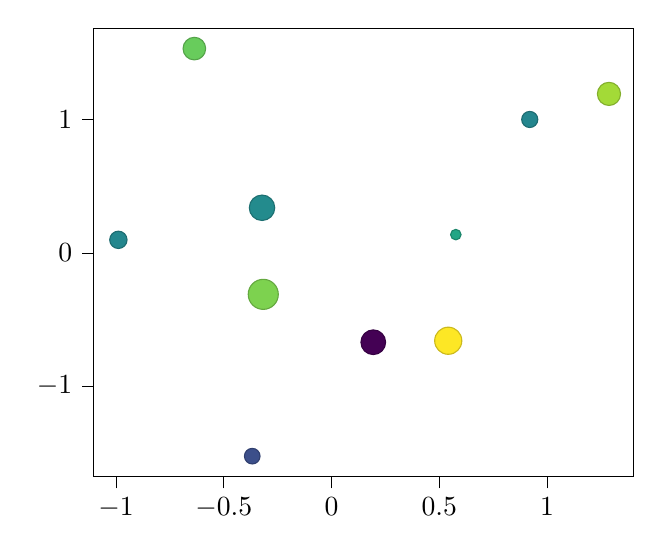
\begin{tikzpicture}

\definecolor{darkgray176}{RGB}{176,176,176}
\definecolor{steelblue31119180}{RGB}{31,119,180}

\begin{axis}[
tick align=outside,
tick pos=left,
x grid style={darkgray176},
xmin=-1.1029737, xmax=1.4017776,
xtick style={color=black},
y grid style={darkgray176},
ymin=-1.6788286, ymax=1.6849313,
ytick style={color=black}
]
\addplot [
  colormap/viridis,
  draw=steelblue31119180,
  mark=*,
  only marks,
  scatter,
  scatter src=explicit,
  scatter/@pre marker code/.append style={/tikz/mark size=\perpointmarksize},
  visualization depends on={\thisrow{sizedata} \as\perpointmarksize}
]
table [x=x, y=y, meta=colordata]{%
x  y  colordata  sizedata
-0.98912135 0.097167319 -0.36176687 3.133158
-0.36778665 -1.5259304 -1.2302322 2.8170726
1.2879253 1.1921661 1.2262293 4.1765659
0.19397442 -0.67108968 -2.1720439 4.4583551
0.9202309 1.0002694 -0.37014735 2.9092943
0.57710379 0.13632112 0.16438007 1.8999492
-0.63646365 1.5320331 0.85988118 4.0841243
0.54195222 -0.65996941 1.7616612 4.9036449
-0.31659545 -0.31179486 0.99332378 5.4313041
-0.32238912 0.33776913 -0.29152143 4.5938359
};
\end{axis}

\end{tikzpicture}
